\chapter{Основная часть}

\section{Постановка задачи}

Разработанная оптимизация метода сжатия страниц памяти заключается в принятии решения о его выполнении на основании вычисленного значения информационной энтропии исходных данных и состоит из следующих этапов:

\begin{enumerate}
	\item Вычисление значения информационной энтропии с помощью метода подсчета.
	\item Сравнение вычисленного значения информационной энтропии с пороговым значением.
	\item Сжатие данных страницы в случае, если полученное значение информационной энтропии меньше порогового значения.
\end{enumerate}

На рисунках \ref{img:zero-level}-\ref{img:first-level} показаны IDEF0-диаграммы нулевого и первого уровней, формализующие поставленную задачу оптимизации метода сжатия страниц памяти с использованием подсчета информационной энтропии.

\begin{figure}[H]
	\begin{center}
		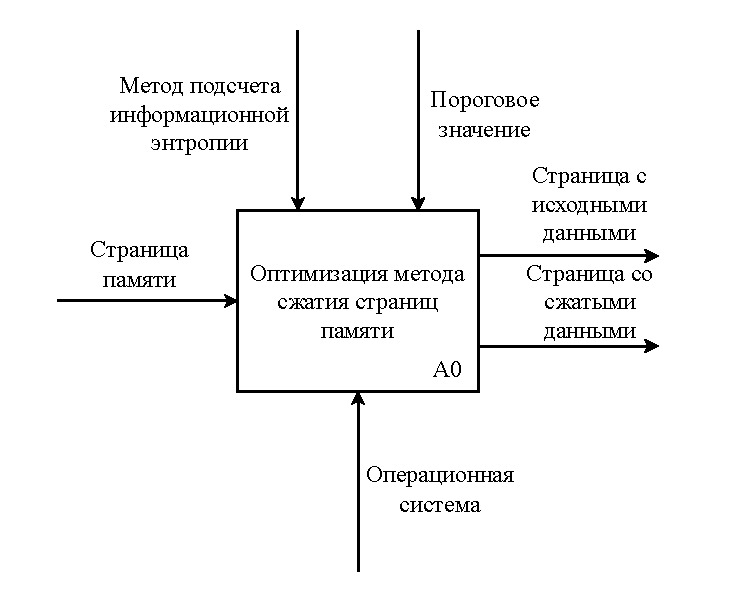
\includegraphics[scale=0.8]{inc/img/zero-level.pdf}
	\end{center}
	\captionsetup{justification=centering}
	\caption{IDEF0-диаграмма нулевого уровня}
	\label{img:zero-level}
\end{figure}

\begin{figure}[H]
	\begin{center}
		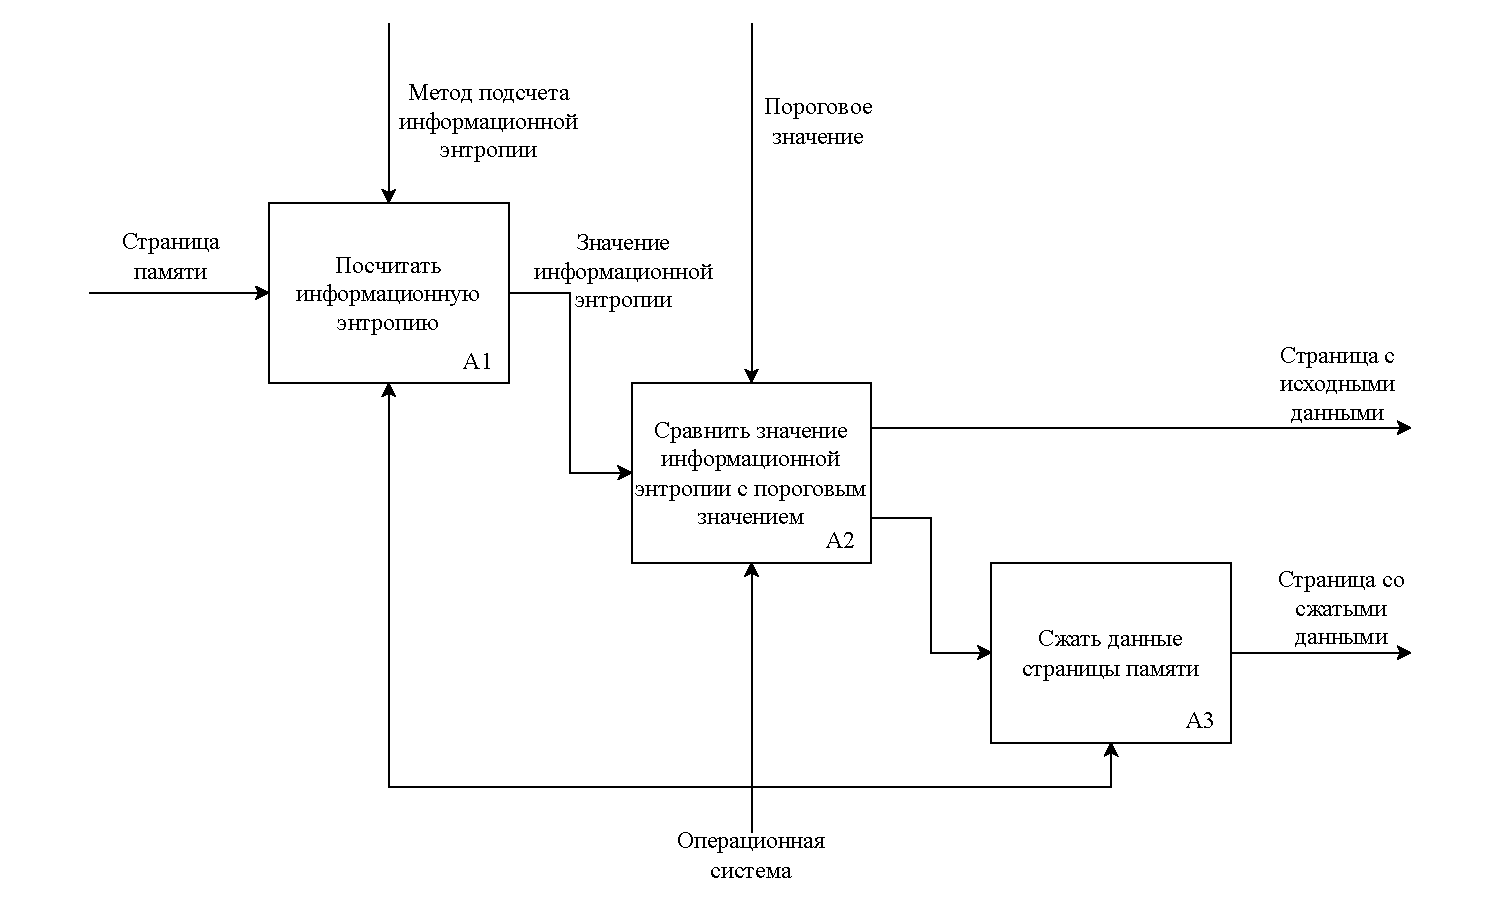
\includegraphics[scale=0.7]{inc/img/first-level.pdf}
	\end{center}
	\captionsetup{justification=centering}
	\caption{IDEF0-диаграмма первого уровня}
	\label{img:first-level}
\end{figure}

Входными данными является страница памяти, которая представляет собой вектор $a = (a_1\text{ }a_2\text{ }\dotso\text{ }a_N)$ размером $N$, равным размеру страницы памяти. При этом, $0 \leq a_i \leq 255$.

На принятие решения о выполнении сжатия влияет сравнение подсчитанного значения информационной энтропии с пороговым значением. Сжатие страниц памяти выполняется ядром операционной системы.

В зависимости от принятого решения выходными данными могут быть:
\begin{itemize}
	\item страница памяти со сжатыми исходными данными, которая представляет собой вектор $b = (b_1\text{ }b_2\text{ }\dotso\text{ }b_N)$ размером $N$, $0 \leq b_i \leq 255$;
    \item страница памяти с исходными данными, которая представляет собой вектор $a$.
\end{itemize}

\section{Требования к программному обеспечению}

Согласно формальному описанию постановки задачи программное обеспечение должно:

\begin{itemize}
	\item вычислять информационную энтропию страницы оперативной памяти, которая является вектором $a = (a_1\text{ }a_2\text{ }\dotso\text{ }a_N)$ размером $N$, равным размеру страницы памяти, $0 \leq a_i \leq 255$;
	\item если вычисленное значение меньше порогового, сжимать данные входной страницы память, то есть, получать вектор $b = (b_1\text{ }b_2\text{ }\dotso\text{ }b_N)$ размером $N$, $0 \leq b_i \leq 255$;
	\item если вычисленное значение больше или равно пороговому, данные входной страницы памяти не должны изменяться;
    \item выполняться как часть ядра операционной системы.
\end{itemize}

\section{Выбор операционной системы}

Программное обеспечение должно выполняться как часть ядра операционной системы, удовлетворяющей следующим критериям:

\begin{itemize}
	\item поддержка сжатия страниц оперативной памяти;
	\item открытый исходный код.
\end{itemize}

Для сравнения, приведенного в таблице \ref{tab:comparison-os}, были выбраны системы, занимающие наибольшие доли рынка операционных систем \cite{stat}.

\begin{table}[h]
    \caption{Сравнение операционных систем}
    \begin{center}
        \begin{tabular}{|l|l|l|l|}
        		\hline
            \multicolumn{1}{|c}{\textbf{Операционная}} & 
            \multicolumn{1}{|c|}{\textbf{Поддержка}} &
            \multicolumn{1}{c|}{\textbf{Открытый}} &
            \multicolumn{1}{c|}{\textbf{Доля}} \\
            \multicolumn{1}{|c}{\textbf{система}} & 
            \multicolumn{1}{|c|}{\textbf{сжатия}} &
            \multicolumn{1}{c|}{\textbf{исходный код}} &
            \multicolumn{1}{c|}{\textbf{рынка (\%)}} \\ \hline
            Windows &  + & - & 63.13 \\ \hline
            OS X & + & - & 17.78 \\ \hline
            Linux & + & + & 2.83 \\ \hline
            FreeBSD & + & + & 0.01 \\ \hline
        \end{tabular}
    \end{center}
    \label{tab:comparison-os}
\end{table}

В результате сравнения была выбрана операционная системы Linux, так как она удовлетворяет выделенным критериям и занимает долю рынка большую, чем операционная система FreeBSD. Возможность сжатия страниц оперативной памяти в ядре Linux предоставляют загружаемые модули zram и zswap.

\section{Выбор модуля сжатия}

При загрузке модуля zram в оперативной памяти создается блочный специальный файл, который моделирует диск. После загрузки модуля страницы, попадаемые на вход моделируемому диску, сжимаются и хранятся сжатыми. Таким образом, страницы находятся в оперативной памяти в сжатом виде.

Модуль zram обладает следующими преимуществами \cite{zram}:

\begin{itemize}
	\item сокращение использования памяти за счет сжатия страниц;
	\item высокая скорость операций чтения и записи, так как блочный специальный файл создается в оперативной памяти;
    \item возможность выбора алгоритма сжатия, предоставляемого Crypto API~\cite{crypto};
    \item возможность реализации хранения временных файлов в сжатом виде;
    \item возможность реализации кэширования страниц памяти;
    \item возможность использования в качестве устройства подкачки;
    \item возможность записи несжимаемых страниц в резервное хранилище;
    \item возможность повторного сжатия с другим алгоритмом сжатия;
    \item многопоточное сжатие.
\end{itemize}

Модуль zswap работает следующим образом:

\begin{itemize}
    \item перехватывает страницу, находящуюся в процессе выгрузки на устройство подкачки;
    \item осуществляет попытку записать данную страницу в сжатом виде в динамически создаваемый пул оперативной памяти;
    \item если размер пула сжатых страниц достигает предела, страницы вытесняются на устройство подкачки с использованием алгоритма LRU.
\end{itemize}

Модуль zswap обладает следующими преимуществами \cite{zswap}:

\begin{itemize}
	\item сокращение использования памяти за счет сжатия страниц;
	\item высокая скорость операций чтения и записи, так как сжатый пул находится в оперативной памяти;
    \item возможность выбора алгоритма сжатия, предоставляемого Crypto API~\cite{crypto}.
\end{itemize}

В результате обзора загружаемых модулей сжатия ядра Linux был выбран модуль zram в связи с его преимуществами и тем, что для работы модуля zswap нужно устройство подкачки, на которое при полном заполнении пула вытесняются страницы памяти.

\section{Выбор инструментов реализации}

В качестве языка программирования был выбран язык C \cite{c}, так как большая часть исходного кода ядра операционной системы Linux и всех ее модулей написана на данном языке программирования.

Для сборки программного обеспечения выбрана утилита GNU make \cite{make}, так как с помощью данной утилиты осуществляется сборка загружаемых модулей ядра.

\section{Структура программного обеспечения}

Структура загружаемого модуля ядра zram включает в себя следующие части:
\begin{itemize}
	\item модуль блочного устройства, который выполняет функции создания, настройки и удаления дисков, обработки операций записи и чтения страниц и получения статистики;
	\item модуль сжатия, который выполняет функции сжатия и восстановления данных, а также настройку этих операций.
\end{itemize}

Функция сжатия данных, предоставляемая модулем сжатия, вызывается в модуле блочного устройства во время обработки записи страницы на диск, как представлено на рисунке \ref{img:zram-structure}.

\includeimage
    {zram-structure}
    {f}
    {h}
    {0.6\textwidth}
    {Структура модуля zram}

Программное обеспечение разрабатывалось как модификация загружаемого модуля ядра zram операционной системы Linux, поэтому имеет структуру, показанную на рисунке \ref{img:structure}.

\begin{figure}[H]
	\begin{center}
		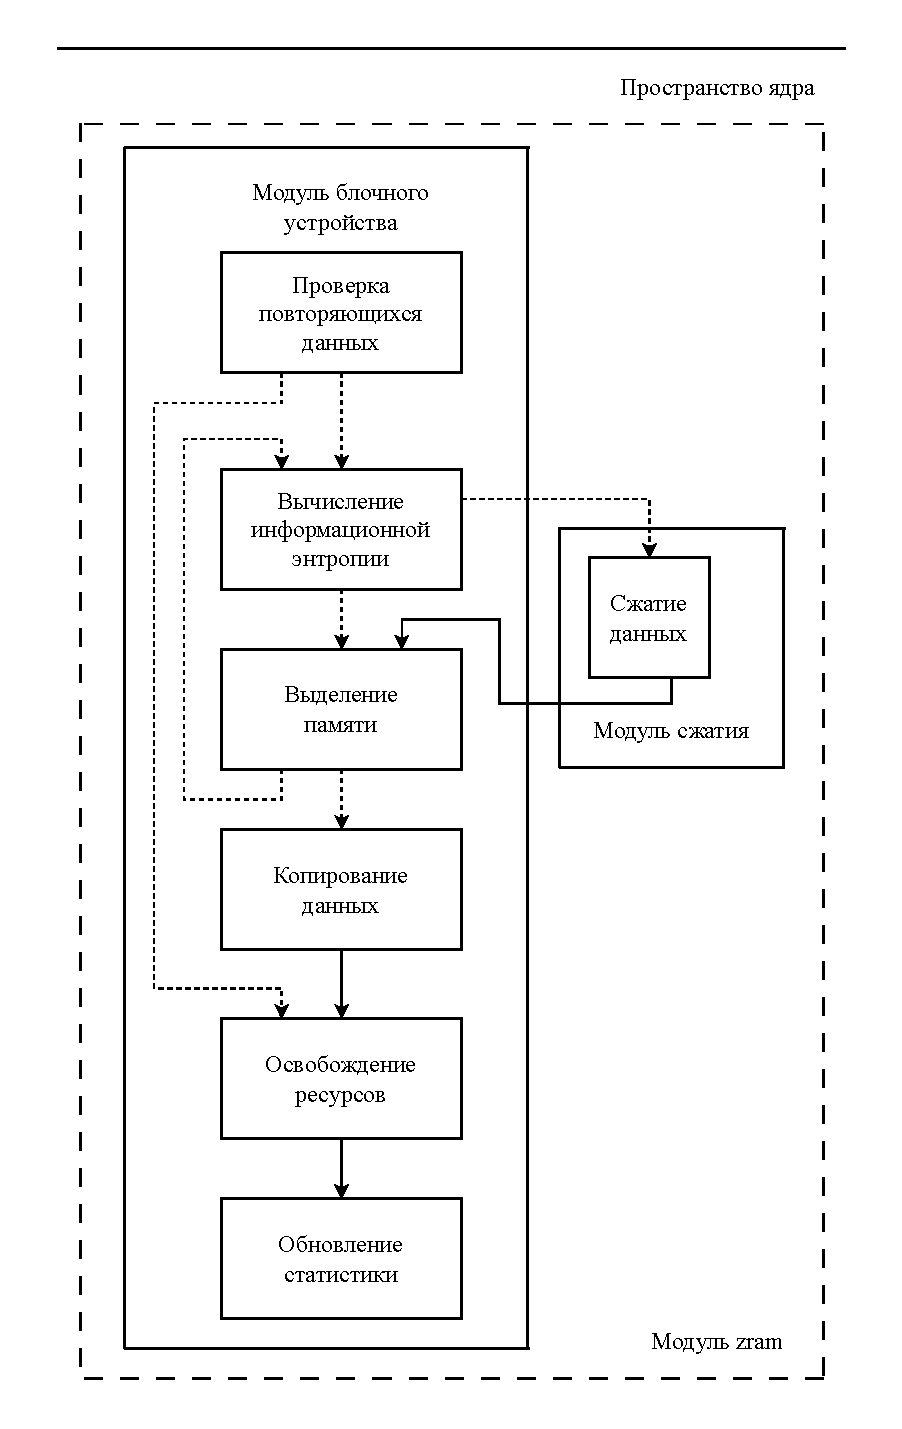
\includegraphics[scale=0.7]{inc/img/structure.pdf}
	\end{center}
	\captionsetup{justification=centering}
	\caption{Структура программного обеспечения}
	\label{img:structure}
\end{figure}

\section{Детали реализации}

В листинге \ref{lst:get_sw_entropy.c} показана реализация метода скользящего окна для подсчета информационной энтропии. Размер страницы в байтах в ядре Linux определяется константой PAGE\_SIZE \cite{block-file}.

\includelistingpretty
    {get_sw_entropy.c}
    {C}
    {Реализация метода скользящего окна для подсчета информационной энтропии}

В листинге \ref{lst:write_page.c} приведена часть реализации записи страницы на диск в модуле блочного устройства.

\includelistingpretty
    {write_page.c}
    {C}
    {Часть реализация записи страницы на диск}

\section{Конфигурация программного обеспечения}

Для сборки, запуска и настройки программного обеспечения был написан make-файл, код которого представлен в листинге \ref{lst:Makefile}.

\includelistingpretty
    {Makefile}
    {C}
    {Конфигурационный файл}

Конфигурационный файл предоставляет следующие возможности для работы с программным обеспечением:

\begin{itemize}
    \item получить исполняемый файл программного обеспечения --- загружаемый модуль, с помощью команды make;
    \item загрузить полученный модуль с помощью команды make load;
    \item проверить, что модуль загружен, с помощью команды make info;
    \item получить сообщения модуля в системном журнале с помощью команды make info;
    \item выгрузить модуль с помощью команды make unload.
\end{itemize}

Средствами конфигурационного файла можно выполнять следующие действия с диском zram:

\begin{enumerate}
    \item Добавить диск с помощью команды make add-disk, в результате выполнения которой на экран будет выведен идентификатор добавленного устройства или код ошибки.
    \item Получить список доступных алгоритмов сжатия для диска с идентификатором i с помощью команды make get-comp-algorithm id=i.
    \item Установить алгоритм сжатия a для диска с идентификатором i с помощью команды make set-comp-algorithm comp-algoritm=a id=i.
    \item Установить размер s диска с идентификатором i с помощью команды make set-disksize disksize=s id=i. Для указания единиц измерения используются следующие постфиксы: K --- размер в килобайтах, M --- размер в мегабайт, G --- размер в гигабайтах. При отсутствии постфикса устанавливается размер в байтах.
    \item Получить статистику памяти диска с идентификатором i с помощью команды make memory-stat id=i.
    \item Освободить память, выделенную для диска с идентификатором i, и сбросить его размер диска до нуля с помощью команды make reset-disk id=i.
    \item Удалить диск с идентификатором i с помощью команды make remove-disk id=i.
\end{enumerate}

\section{Пример работы программного обеспечения}

На рисунке \ref{img:example} показана часть статистики обработки программным обеспечением страниц файлов с расширениями .h и .c.

\begin{figure}[H]
	\begin{center}
		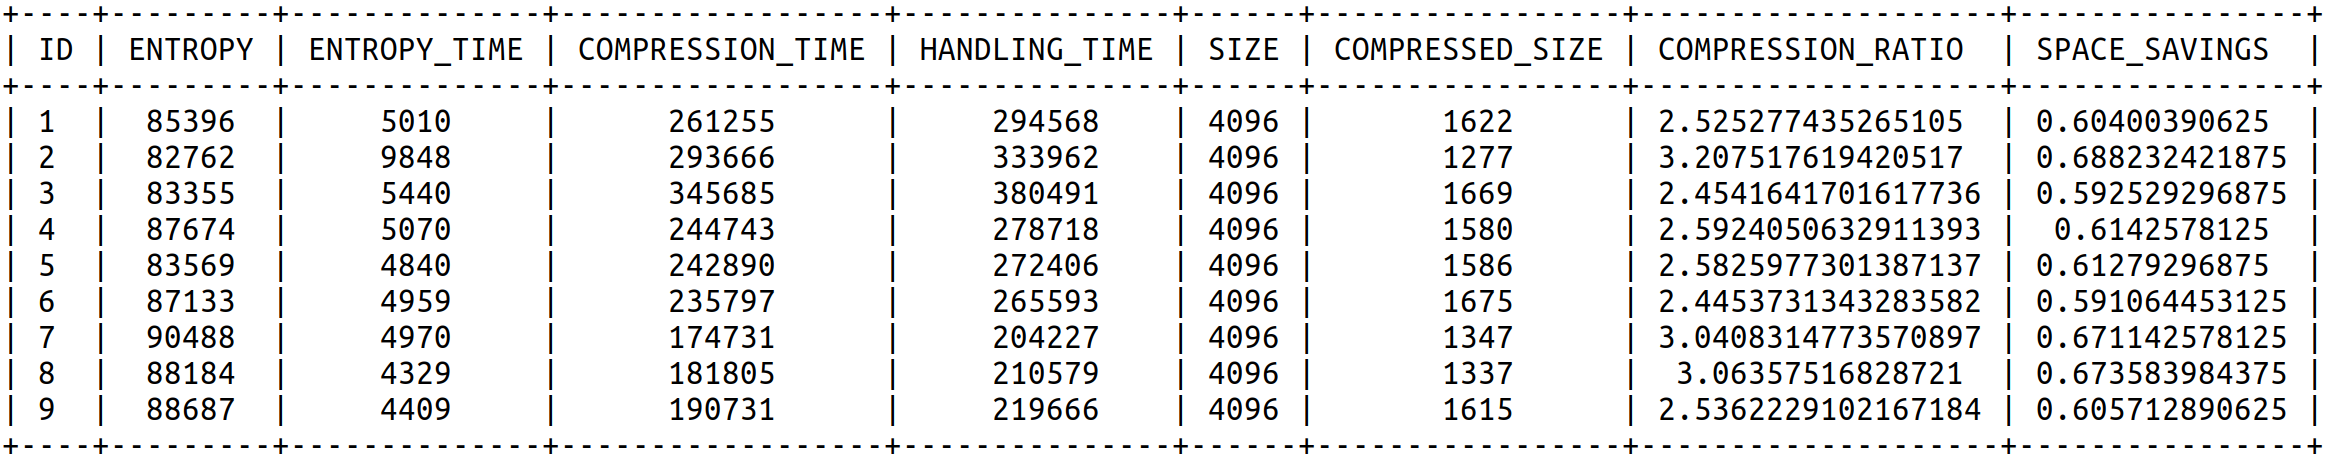
\includegraphics[scale=0.25]{inc/img/example.png}
	\end{center}
	\captionsetup{justification=centering}
	\caption{Часть статистики обработки страниц файлов с расширениями .h и .c}
	\label{img:example}
\end{figure}

Данные статистики оформлены в виде таблицы со следующими столбцами:

\begin{itemize}
    \item ID --- идентификатор страницы, соответствующий номеру страницы в порядке их обработки;
    \item ENTROPY --- значение информационной энтропии исходных данных страницы;
    \item ENTROPY\_TIME --- время вычисления информационной энтропии в наносекундах;
    \item COMPRESSION\_TIME --- время сжатия данных страницы в наносекундах;
    \item HANDLING\_TIME --- время обработки страницы в наносекундах, равное времени выполнения функции записи страницы на диск;
    \item SIZE --- размер исходных данных в байтах;
    \item COMRESSED\_SIZE --- размер сжатых данных в байтах;
    \item COMPRESSION\_RATIO --- отношение объема исходных данных к объему сжатых данных;
    \item SPACE\_SAVINGS --- уменьшение размера файла по сравнению с размером несжатого файла.
\end{itemize}